\documentclass[10pt]{beamer}
\synctex=1
\usepackage{amsmath,amsthm, amssymb, amsfonts, mathrsfs}
% \usepackage[pagebackref=true]{hyperref}
\usetheme[progressbar=frametitle,block=fill]{metropolis}
\metroset{block=fill}
\setbeamercolor{progress bar in head}{fg=red}
\usepackage{mathabx,epsfig}
\def\acts{\mathrel{\reflectbox{$\righttoleftarrow$}}}
\usepackage{cleveref, xcolor, bbm, array,
  esint,nicefrac,tikz-cd,tikz,enumitem, subcaption, wrapfig}
% \usetikzlibrary{patterns}
\usepackage[toc,page]{appendix}
\usepackage{physics}
%\usepackage[protrusion=true,expansion=true]{microtype}
\usepackage{natbib}
% \usepackage[nottoc]{tocbibind}
% \usepackage{wrapfig}
\usepackage{float} 
% \usepackage{kpfonts}
% \usepackage[utf8]{inputenc}
% \usepackage[T1]{fontenc}
% \usepackage{yfonts}
% \usepackage{kpfonts,fontspec}
% \usepackage[math-style=ISO, bold-style=ISO]{unicode-math}

% \setmathfont{Garamond-Math.otf}

% \usepackage[urw-garamond]{mathdesign}
% \usepackage{garamondx}
% \usepackage{newtxmath}
%\usepackage{lmodern}

% \usepackage{CormorantGaramond}
%\setmathfont{Garamond-Math.otf}[StylisticSet={7,9}]

% \usepackage{minitoc, tocloft}

% \usepackage[margin=1in]{geometry}
%\usepackage[right= 4.5cm, left=4.5cm, top= 2.5cm, bottom=2.0cm]{geometry}

% \pagenumbering{gobble} 
% \setenumerate{noitemsep}


\let\mbb\mathbb
\let\mscr\mathscr
\let\mc\mathcal
\let\mf\mathfrak
\let\mbf\mathbf

\newcommand{\pur}[1]{{\color{purple!45!black} #1}}
\newcommand{\ps}[1]{[\![#1]\! ]}
\newcommand{\A}{\mathbb{A}}
\newcommand{\N}{\mathbb{N}}
\newcommand{\Z}{\mathbb{Z}}
\newcommand{\Q}{\mathbb{Q}}
\newcommand{\R}{\mathbb{R}}
\newcommand{\C}{\mathbb{C}}
\renewcommand{\P}{\mathbb{P}}
\renewcommand{\H}{\textfrak{H}}
\renewcommand{\O}{\mathcal{O}}
\newcommand{\Ca}{\mathscr{C}}
\newcommand{\F}{\mbb{F}}
\renewcommand{\L}{\mathscr{L}}
\newcommand{\p}{\mathfrak{p}}
\newcommand{\Lip}{\mathrm{Lip}\,}
\newcommand{\lav}{\mathrm{Lav}}
\newcommand{\Lav}{\mathrm{Lav}}
\newcommand{\loc}{\text{loc}}
\newcommand{\nsub}{\trianglelefteq}
\newcommand{\Set}{\mathbf{Set}}
\newcommand{\Ab}{\mathbf{Ab}}
\newcommand{\Sc}{\mathbf{Sc}}
\newcommand{\Aff}{\mathbf{Aff}}
\newcommand{\Coh}{\mathbf{Coh}}
\newcommand{\Ring}{\mathbf{Ring}}
\newcommand{\Comp}{\mathbf{Comp}}
\newcommand{\Mod}{\mathbf{Mod}}
\newcommand{\pow}[1]{[\![#1]\!]}
% \newcommand{\norm}[2]{\left\lVert #1 \right\rVert_{#2}}
\newcommand{\Norm}[1]{\left\lVert #1 \right\rVert}
\newcommand*{\defeq}{\mathrel{\vcenter{\baselineskip0.5ex \lineskiplimit0pt
      \hbox{\scriptsize.}\hbox{\scriptsize.}}}%
  =}

\newcommand\labelenumi{\textnormal{(\Roman{enumi})}}
\renewcommand\theenumi\labelenumi
\newcommand{\labelitemi}{$\circ$}
\newcommand{\labelitemii}{$\diamond$}
% \renewcommand{\qedsymbol}{$\blacksquare$ \\} 
\renewcommand{\setminus}{\smallsetminus}
\renewcommand{\bar}{\overline}
\renewcommand{\tilde}{\widetilde}
% \renewcommand{\phi}{\varphi}
\renewcommand{\theta}{\vartheta}
\renewcommand{\emptyset}{\varnothing}
\renewcommand{\op}{\text{op}}
\newcommand{\ls}[2]{\qty(\frac{#1}{#2})}

\renewcommand{\arraystretch}{2}
%\renewcommand{\cftsecfont}{\small}

\DeclareMathOperator{\supp}{supp}
\DeclareMathOperator{\ord}{ord}
\DeclareMathOperator{\Nm}{Nm}
\DeclareMathOperator{\Reg}{Reg}
% \DeclareMathOperator{\Res}
\DeclareMathOperator*{\esssup}{ess\,sup}
\DeclareMathOperator{\spn}{span}
\DeclareMathOperator{\Sl}{Sl}
\DeclareMathOperator{\Gl}{Gl}
\DeclareMathOperator{\GL}{GL} 
\DeclareMathOperator{\Id}{Id}
\DeclareMathOperator{\Aut}{Aut}
\DeclareMathOperator{\Hom}{Hom}
\DeclareMathOperator{\Gal}{Gal}
\DeclareMathOperator{\Pic}{Pic}
\DeclareMathOperator{\Char}{char}
\DeclareMathOperator{\AC}{AC}
\DeclareMathOperator{\OP}{OP}
\DeclareMathOperator{\pSh}{pSh}
\DeclareMathOperator{\Sh}{Sh}
\DeclareMathOperator{\Spec}{Spec}
\DeclareMathOperator{\Fun}{Fun}
\DeclareMathOperator{\im}{Im}
\DeclareMathOperator{\et}{\acute{e}t}
\DeclareMathOperator{\Cl}{Cl}
% \theoremstyle{plain}
% \newtheorem{thm}{Theorem}[section]
% \newtheorem{cor}[thm]{Corollary}
% \newtheorem*{conj}{Question}
% \newtheorem{lemma}[thm]{Lemma}
% \newtheorem{prop}[thm]{Proposition}
% \theoremstyle{definition}
% \newtheorem{mydef}[thm]{Definition}
% \newtheorem{example}[thm]{Example}
% \newtheorem{non-example}[thm]{Non-example}
% \theoremstyle{remark}
% \newtheorem*{remark}{Remark}
% \theoremstyle{definition}
% \newtheorem{exercise}{Exercise}
% \numberwithin{equation}{section}

\hypersetup{
  colorlinks,
  linkcolor={red!50!black},
  citecolor={purple!45!black},
  urlcolor={green!40!black}
}
\makeatletter
\newcommand{\Pause}[1][]{\unless\ifmeasuring@\relax
\pause[#1]%
\fi}
\makeatother

\begin{document}
\title{Computing $p$-adic $L$-functions \\ \normalsize of Hecke characters}
\author{Håvard Damm-Johnsen}
\date{\today}
\institute{University of Oxford \\ Junior number theory seminar}

\maketitle
\begin{frame}
  \frametitle{Outline}

  \begin{itemize}[itemsep=5pt]
  \item \textbf{$L$-functions}: a $5$-min elevator pitch\pause
    
  \item \textbf{$p$-adic $L$-functions}: a quick intro \pause

  \item \textbf{Algorithm}: computing $p$-adic $L$-functions on a machine\pause

  \item \textbf{Data}: some explicit $p$-adic $L$-functions\pause

  \item \textbf{Applications \& extensions}     
  \end{itemize}

  
\end{frame}

\section{$L$-functions}
\begin{frame}{What is an $L$-function?}
\begin{itemize}[leftmargin=2pt]\pause
\item Prototype: the Riemann zeta function $\zeta(s) = \sum_{n=1}^{\infty}\frac{1}{n^{s}}$.\pause
\begin{itemize}
\item Euler product: $\zeta(s) = \prod_{p} (1-p^{-s})^{-1}$\pause
\item Functional equation:
  \[     \xi(s) = \xi(1-s) \qq{where} \xi(s) \defeq
  \pi^{-s/2}\frac{s(s-1)}{2} \Gamma\qty(\frac{s}{2})\zeta(s) \vspace{-10pt}\pause
  \]
\item Meromorphic continuation, $\zeta \colon \C \to \C$ \pause
\item Fundamental in analytic number theory (eg. PNT)  \pause
\end{itemize}
\item \textbf{Selberg class $L$-function}: Dirichlet series
  $\sum_{n}\frac{a_{n}}{n^{s}}$ satisfying the above + growth condition
  on $a_{n}$.
\end{itemize}
  \begin{figure}[H]
  \centering
  \begin{subfigure}[b]{0.3\textwidth}
  \centering
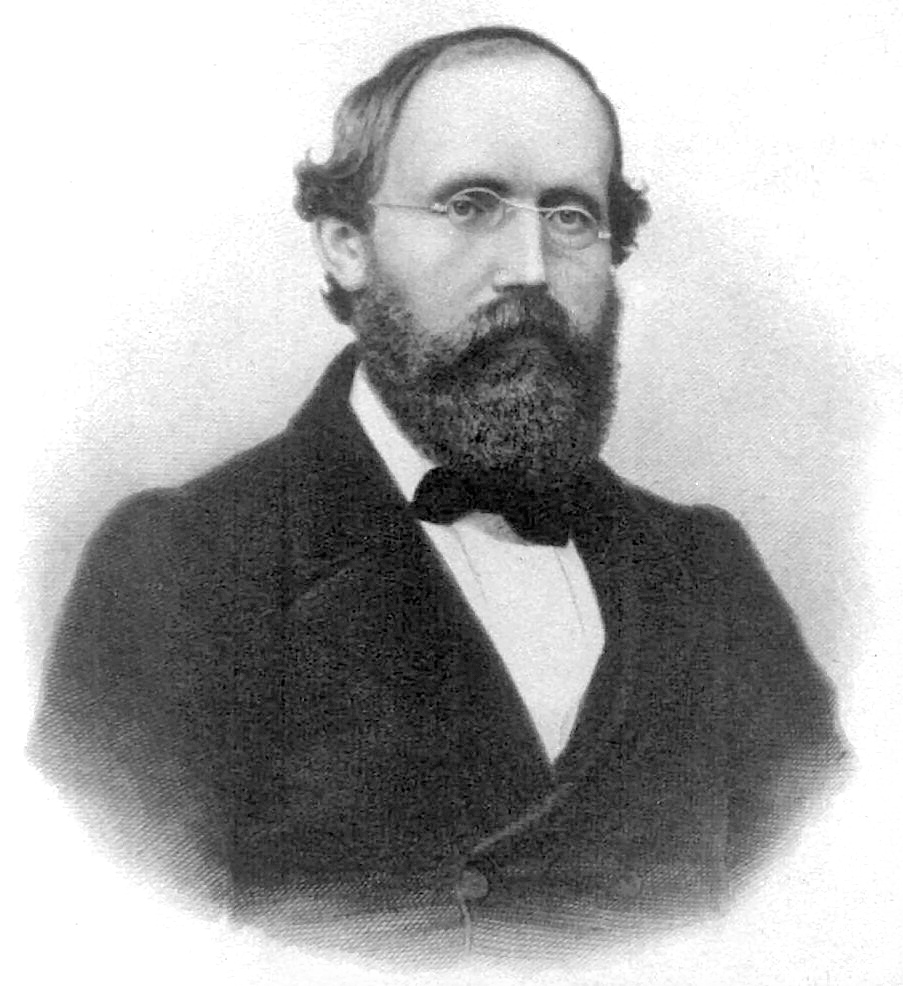
\includegraphics[width=.6\textwidth]{Riemann.jpeg}
\end{subfigure}
  \begin{subfigure}[b]{0.3\textwidth}
  \centering
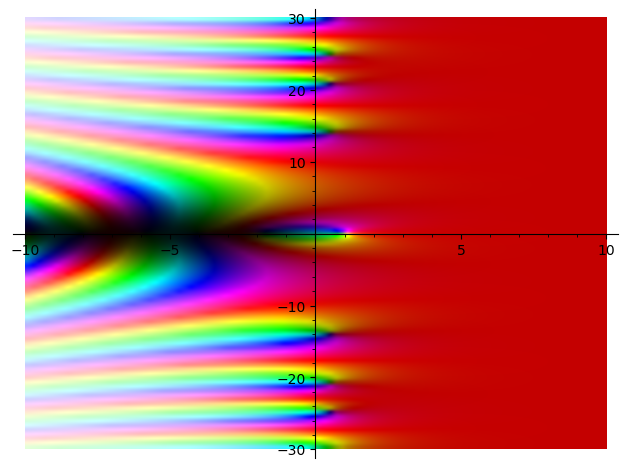
\includegraphics[width=.9\textwidth]{zeta-plot2.png}
\end{subfigure}
  \begin{subfigure}[b]{0.3\textwidth}
  \centering
\includegraphics[width=.7\textwidth]{Selberg.jpg}
\end{subfigure}
\end{figure}\vspace{-5pt}


\end{frame}


\begin{frame}{Dirichlet $L$-functions}
\begin{itemize}[leftmargin=2pt]
\item Let $\chi \colon \Z \to \C^{\times}$ be a Dirichlet character of modulus
  $N$ (i.e. a periodic multiplicative function of period $N$).\pause
\item The \textbf{Dirichlet $L$-function} $L(\chi,s)\defeq
  \sum_{n=1}^{\infty}\frac{\chi(n)}{n^{s}}$ is Selberg class. \pause
\item $S \defeq \{a + bn : n \in \Z\}$, $a,b \in \N$; write
  $\mathbbm{1}_{S}$ as a linear combo of Dirichlet characters to prove
  that $S$ contains infinitely many primes.\pause
\item By viewing $\chi$ as a $1$-dim. rep. $\Gal(\Q(\zeta_{N}))\to \C^{\times}= \Gl_{1}(\C)$, this
  generalises to \textbf{Artin $L$-functions} attached to representations.
\end{itemize}\vspace{-5pt}

  \begin{figure}[H]
  \centering
  \begin{subfigure}[b]{0.3\textwidth}
  \centering
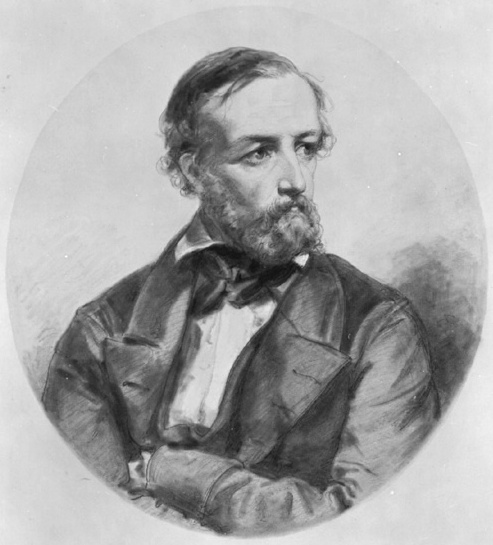
\includegraphics[width=.6\textwidth]{Dirichlet.jpg}
\end{subfigure}
  \begin{subfigure}[b]{0.3\textwidth}
  \centering
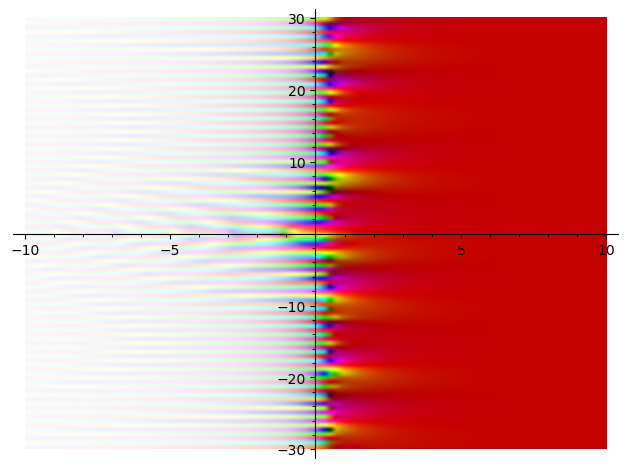
\includegraphics[width=\textwidth]{DirichletLfunction67.png}
\end{subfigure}
  \begin{subfigure}[b]{0.3\textwidth}
  \centering
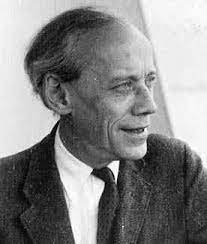
\includegraphics[width=.7\textwidth]{EArtin.jpeg}
\end{subfigure}
\end{figure}\vspace{-5pt}

\end{frame}
\begin{frame}{Zeta functions of number fields}

  \begin{itemize}[leftmargin=2pt]
  \item  Fix $F$ a number field with ring of integers $\O_{F}$.  \pause
  \item e.g. $F = \Q(\sqrt{3}) = \{ a+b\sqrt{3} : a,b \in
\Q\}$, $\O_{F} = \Z + \sqrt{3}\Z$.\pause
\item ``Natural'' generalisation of $\Q,\Z$. \pause
\item \textbf{Dedekind zeta function}: $\zeta_{F}(s)\defeq \sum_{\mf a \leq
    \O_{F}}\frac{1}{\Nm(\mf a)^{s}}$. \pause
\item Has meromorphic cont., Euler product and functional eqn.\pause
\item  Dirichlet class number formula: \pause
    \[ \Res_{s=1}\zeta_{F}(s)= \frac{2^{r_{1}}(2\pi)^{r_{2}}\Reg_{F}h_{F}
      }{w_{F}\sqrt{|\Delta_{F}|}} \] \pause
\item Dedekind's conjecture: given $F'/F$, the function $\zeta_{F'}(s)/\zeta_{F}(s)$ is entire
  \end{itemize}\vspace{-5pt}

  \begin{figure}[H]
  \centering
  \begin{subfigure}[b]{0.3\textwidth}
  \centering
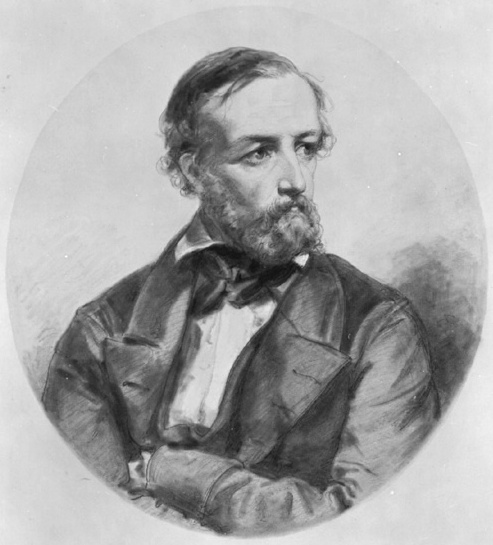
\includegraphics[width=.6\textwidth]{Dirichlet.jpg}
\end{subfigure}
  \begin{subfigure}[b]{0.3\textwidth}
  \centering
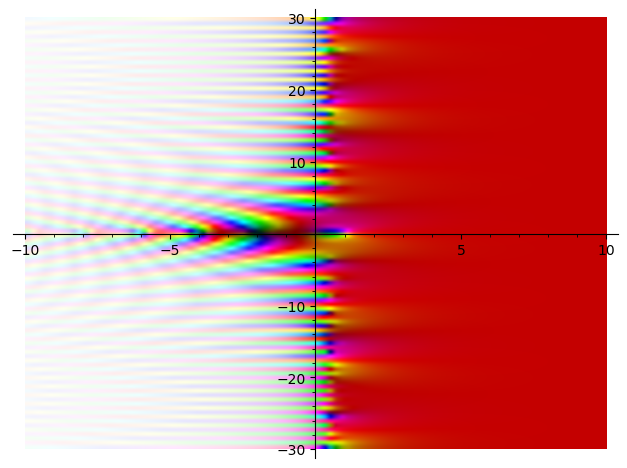
\includegraphics[width=\textwidth]{Fzeta-plot.png}
\end{subfigure}
  \begin{subfigure}[b]{0.3\textwidth}
  \centering
\includegraphics[width=.5\textwidth]{Dedekind.jpg}
\end{subfigure}
\end{figure}\vspace{-5pt}

\end{frame}

\begin{frame}{$L$-functions over number fields}
  \begin{itemize}
  \item Generalise Dirichlet $L$-functions: need ``Dirichlet
    characters of ideals''\pause
  \item Hecke characters: $\chi \colon \Cl_{\mf m}(F)\to\C^{\times}$\pause
  \item \textbf{Hecke $L$-function}: $L(\chi,s) \defeq \sum_{\mf a \leq
      \O_{F}}\frac{\chi(\mf a)}{\Nm(\mf a)^{s}}$\pause
  \item Has meromorphic cont., Euler product and functional eqn.\pause
  \item Natural interpretation using \emph{adèles}, cf. Tate's thesis\pause
  \end{itemize}
    \begin{figure}[H]
  \centering
  \begin{subfigure}[b]{0.3\textwidth}
  \centering
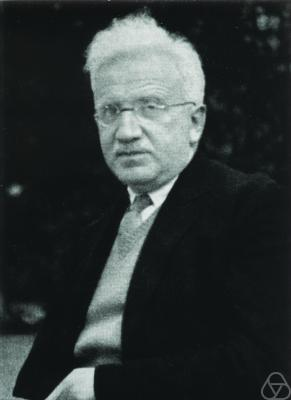
\includegraphics[width=.6\textwidth]{Hecke.jpg}
\end{subfigure}
  \begin{subfigure}[b]{0.3\textwidth}
  \centering
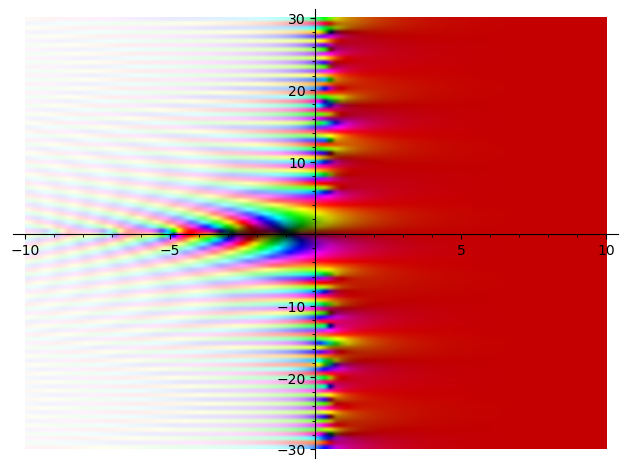
\includegraphics[width=\textwidth]{Hzeta-plot.png}
\end{subfigure}
  \begin{subfigure}[b]{0.3\textwidth}
  \centering
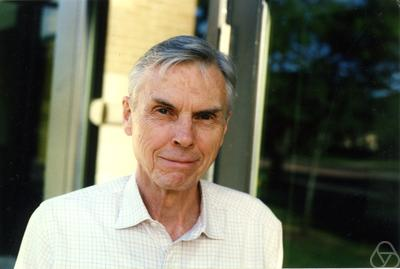
\includegraphics[width=.9\textwidth]{Tate.jpg}
\end{subfigure}
\end{figure}\vspace{-5pt}
\end{frame}


\begin{frame}{Other $L$-functions}
Can attach $L$-functions to other objects, e.g. varieties or reps\pause
  \begin{itemize}[leftmargin=2pt]

\item $L(X,s)$ - meromorphic functions ``built from local data''\pause 
\item Special value formulae: analogues of Dirichlet class number
  formula
      \[ \Res_{s=1}\zeta_{F}(s)= \frac{2^{r_{1}}(2\pi)^{r_{2}}\Reg_{F}h_{F}
        }{w_{F}\sqrt{|\Delta_{F}|}} \]\pause
\begin{itemize}
\item $X = $ number field: Stark conjectures \pause
  \item $X = $ elliptic curve: BSD conjecture, Gross-Zagier formula\pause
  \item $X = $ algebraic variety: Conjectures of Bloch, Beilinson,
    Deligne, ... \pause 
  \end{itemize}
\item \emph{$p$-adic $L$-functions}: 
  $L_{p}(X,s) \colon \Z_{p}\to \C_{p}$ - interpolates special values of
  $L(X,s)$ \pause 
\begin{itemize}
\item Starting point of Iwasawa theory\pause
\item Iwasawa main conjectures \pause
\item $p$-adic BSD conjecture
\end{itemize} 
\end{itemize}

\end{frame}
\section{$p$-adic $L$-functions}
\begin{frame}
  \frametitle{$p$-adic $L$-functions over $\Q$}
\begin{itemize}\pause

\item \textbf{Euler + functional equation:} for $k$ even, $\zeta(1-k) = -B_{k}/k$.\pause
\item \textbf{Kummer:} if $k \equiv k' \mod{(p-1)p^{N}}$ are even, then
  \[   (1-p^{k-1})\frac{B_{k}}{k} \equiv (1-p^{k'-1})\frac{B_{k'}}{k'} \mod{p^{N}}.\pause
  \]
\vspace{-5pt}
\item By $p$-adic analysis, if
  $k_{0}\equiv k_{1}\equiv \ldots \mod{p-1}$, then $(1-p^{k_{i}-1})\zeta(1-k_{i})$ interpolate to
  $\zeta_{p}\colon \Z_{p}\to \C_{p}$. \pause
\item different ``branches'' corresponding to $\bar k_{0} \in \Z/(p-1)\Z$.\pause
\item We can approximate $\zeta_{p}(s)$ by computing $\zeta(1-k)$ for
  enough $k$ and use polynomial interpolation: \pause

\item given pairs
  $\{(1-k_{i},\zeta_{p}(1-k_{i})) : i = 1,\ldots, d\}$, find a polynomial
  $P$ of degree $d$ such that $P(1-k_{i}) = \zeta_{p}(1-k_{i})$. \pause
\item \textbf{Eg.} $p=5, k_{i}\in \{2,6,10\}$, interpolate $\{(k_{i},-(1-5^{k_{i}-1})B_{k_{i}}/k_{i})\}$: \pause
  \[\left(5^{2} \cdot 4828 + O(5^{8})\right) s^{2} + \left(5 \cdot 60514 + O(5^{8})\right) s + 51662 + O(5^{8})\pause \ ``\approx"  \ \zeta_{5}(s)
  \]
\end{itemize}

\end{frame}




\begin{frame}
  \frametitle{$p$-adic $L$-functions over $F$}
\begin{itemize}[leftmargin=2pt]\pause
\item Fix $F$ a \emph{totally real} number field of degree $d$, $\psi$ a
  character of $\Cl_{\mf m}^{+}$. \pause
\item Define $L(\psi,s) \defeq \sum_{\mf a \le \O_{F}} \frac{\psi(\mf a)}{\Nm(\mf
    a)^{s}}$; \pause then
  $L(\psi,1-k) = -B_{k,\psi}/k \in \bar \Q$.\pause
\item Interpolation: $L_{p}(\psi,1-k) = (1-\psi(p)p^{k-1})L(\psi,1-k)$. \pause
\item However, not obvious how to compute $B_{k,\psi}$ algebraically \emph{quickly}, so
  we need a new strategy! \pause
\item \textbf{Serre (Antwerp III):} The modular form
  \[ G_{k}^{*} = \frac{1}{2} \zeta_{p}(1-k) + \sum_{n=1}^{\infty}\qty(\sum_{d \mid n,\,
    (d,p)=1}d^{k-1})q^{n}
  \]
  on $\Gamma_{0}(p)$ lives in a $p$-adically continuous family of $G_{k_{i}}$. \pause
\item Congruences between non-constant terms gives congruences between
  the constant terms, in fact, the Kummer congruences.
\end{itemize}
% (More details can be found in a preprint by Lauder-Vonk)
\end{frame}

\begin{frame}{$p$-adic $L$-functions from modular forms}
\begin{itemize}[leftmargin=-3pt]
\item \textbf{Idea:} look for modular forms with constant term $L(\psi,1-k)$.\pause
% \item  A \textbf{Hilbert modular form} is a function $f \colon \mf h^{d} \to
%   \C$ which ``transforms like a modular form'' under
%   $\Sl_{2}(\O_{F}) \acts \mf h^{d}$.\pause
\item There is a \emph{Hilbert modular form} $G_{k,\psi}^{(p)}\colon \mf
  h^{d}\to \C$ defined as  
  \[ \hspace{-10pt}G_{k,\psi}^{(p)}(z_{1},\ldots, z_{d}) = L_{p}(\psi,1-k) + 2^{d}\sum_{\nu \in \mf
      d^{-1}_{+}}\Big(\!\sum_{\substack{\mf a \mid (\nu)\mf d \\ (\mf a, p) =
        1}}\psi(\mf a)\Nm(\mf a)^{k-1}\!\Big)e^{2\pi i (\sigma_{1}(\nu)z_{1} + \ldots
      \sigma_{d}(\nu)z_{d})}. \pause
  \]
  
% \item \textbf{Deligne-Ribet:} the ``Hilbert Eisenstein series'',
%   \[ \hspace{-10pt}G_{k,\psi}^{(p)}(z_{1},\ldots, z_{d}) = L_{p}(\psi,1-k) + 2^{d}\sum_{\nu \in \mf
%       d^{-1}}\Big(\!\sum_{\substack{\mf a \mid (\nu)\mf d \\ (\mf a, p) =
%         1}}\psi(\mf a)N(\mf a)^{k-1}\!\Big)e^{2\pi i (\sigma_{1}(\nu)z_{1} + \ldots \sigma_{d}(\nu)z_{d})}
%   \]

\item Setting $z_{1} = \ldots = z_{d} = z$, we get the \textbf{diagonal restriction}
  \[\Delta_{k,\psi}(z) = L_{p}(\psi,1-k) + 2^{d}\sum_{n>0}\sum_{\substack{ \nu \in \mf
      d^{-1}_{+}\\ \tr(\nu) = n}}\Big(\!\sum_{\substack{\mf a \mid (\nu)\mf d \\ (\mf a, p) =
        1}}\psi(\mf a)\Nm(\mf a)^{k-1}\!\Big)q^{n}\pause
  \]
\item This is a classical modular form of weight $dk$. \pause
\item \textbf{Key idea:} knowing a basis for $M_{dk}$ and enough
   coefficients of
  $\Delta_{k,\psi}(z)$ lets us solve for $L_{p}(\psi,1-k)$!
\end{itemize}

\end{frame}
\section{Algorithm}
\begin{frame}
  \frametitle{Algorithm [Lauder-Vonk21]}\pause
  \textbf{Input:}\pause
  \begin{itemize}[itemsep=0pt,leftmargin=0pt]
  \item $F$ totally real number field,\pause
  \item $p$ prime,\pause
  \item $k_0 \in \Z $ ``starting weight'', $m \in \N$ ``precision'',\pause
  \item  $\psi \colon \Cl_{\mf m}^{+}(F)\to \C^{\times}$, $(M) \defeq \mf m \cap \Z$ \pause
  \end{itemize}

 \textbf{Output:} $L_p(\psi,s)$ as an element of $\O_{F}[s]/(p^m)$. \pause

 \begin{enumerate}[leftmargin=2pt]
 \item Set interpolation weights $k_{j} = k_{0} + j(p-1)$, \pause  compute
   bases for $M_{dk_{j}}(\Gamma_{0}(M),\psi)$ for $j =1, \ldots ,\delta_{m} \approx m$.\pause
 \item Compute non-constant coefficients of $\Delta_{k_{j},\psi}$:
   \[ a_{n} =\sum_{\substack{ \nu \in \mf
      d^{-1}_{+}\\ \tr(\nu) = n}}\sum_{\substack{\mf a \mid (\nu)\mf d \\ (\mf a, p) =
        1}}\psi(\mf a)\Nm(\mf a)^{k_{j}-1}, \qq{} n>0. \pause
   \]
 \item Write $\Delta_{k_{j},\psi}$ as linear combination of modular forms in
   $M_{dk_{j}}$ and solve for constant term, $L_{p}(\psi,1-k_{j})$. \pause
 \item Interpolate the $\delta_{m}+1$ values of $L_{p}(\psi,1-k_{j})$ to find
   $L_{p}(\psi,s)$.
 \end{enumerate}

\end{frame}

% \begin{frame}
%   \frametitle{Data, $F = \Q(\sqrt{3})$}
%   \tiny
% \begin{tabular}{|p{.02\linewidth}|p{.93\linewidth}|} \hline
% {\small $p$ }&{\small  $L_p(\mbf 1,s) \in \O_{F}[s] \pmod{p^{m}}$} \\ \hline
%   \hline
% $5$ & $O(5^{8}) s^{14} + O(5^{8}) s^{13} + O(5^{8}) s^{12} + O(5^{8}) s^{11} + O(5^{8}) s^{10} + O(5^{8}) s^{9} + O(5^{8}) s^{8} + \left(5^{6} \cdot 12 + O(5^{8})\right) s^{7} + \left(5^{6} \cdot 18 + O(5^{8})\right) s^{6} + \left(5^{4} \cdot 308 + O(5^{8})\right) s^{5} + \left(5^{5} \cdot 12 + O(5^{8})\right) s^{4} + \left(5^{3} \cdot 811 + O(5^{8})\right) s^{3} + \left(5^{3} \cdot 1839 + O(5^{8})\right) s^{2} + \left(5 \cdot 202997 + O(5^{9})\right) s + 8760231 + O(5^{10})$ \\ \hline
% $7$ & $O(7^{9}) s^{12} + O(7^{9}) s^{11} + O(7^{9}) s^{10} + \left(7^{8} \cdot 4 + O(7^{9})\right) s^{9} + \left(7^{7} \cdot 26 + O(7^{9})\right) s^{8} + \left(7^{6} \cdot 339 + O(7^{9})\right) s^{7} + \left(7^{6} \cdot 41 + O(7^{9})\right) s^{6} + \left(7^{5} \cdot 1955 + O(7^{9})\right) s^{5} + \left(7^{4} \cdot 12339 + O(7^{9})\right) s^{4} + \left(7^{3} \cdot 43352 + O(7^{9})\right) s^{3} + \left(7^{2} \cdot 755539 + O(7^{9})\right) s^{2} + \left(7 \cdot 2363400 + O(7^{9})\right) s + 236098386 + O(7^{10})$ \\ \hline
% $11$ & $O(11^{9}) s^{12} + O(11^{9}) s^{11} + O(11^{10}) s^{10} + \left(11^{9} \cdot 7 + O(11^{10})\right) s^{9} + \left(11^{9} \cdot 9 + O(11^{10})\right) s^{8} + \left(11^{7} \cdot 983 + O(11^{10})\right) s^{7} + \left(11^{6} \cdot 2077 + O(11^{10})\right) s^{6} + \left(11^{5} \cdot 99624 + O(11^{10})\right) s^{5} + \left(11^{4} \cdot 874530 + O(11^{10})\right) s^{4} + \left(11^{3} \cdot 15178197 + O(11^{10})\right) s^{3} + \left(11^{2} \cdot 760252 + O(11^{9})\right) s^{2} + \left(11 \cdot 125621362 + O(11^{9})\right) s + 18201420921 + O(11^{10})$ \\ \hline
% $13$ & $O(13^{10}) s^{11} + O(13^{10}) s^{10} + \left(13^{9} \cdot 10 + O(13^{10})\right) s^{9} + \left(13^{8} \cdot 118 + O(13^{10})\right) s^{8} + \left(13^{7} \cdot 811 + O(13^{10})\right) s^{7} + \left(13^{6} \cdot 210 + O(13^{10})\right) s^{6} + \left(13^{5} \cdot 88733 + O(13^{10})\right) s^{5} + \left(13^{4} \cdot 3403408 + O(13^{10})\right) s^{4} + \left(13^{4} \cdot 2585989 + O(13^{10})\right) s^{3} + \left(13^{2} \cdot 84148803 + O(13^{10})\right) s^{2} + \left(13 \cdot 9530516807 + O(13^{10})\right) s + 41080902718 + O(13^{10})$ \\ \hline
% $17$ & $O(17^{10}) s^{11} + O(17^{10}) s^{10} + \left(17^{9} \cdot 10 + O(17^{10})\right) s^{9} + \left(17^{8} \cdot 277 + O(17^{10})\right) s^{8} + \left(17^{7} \cdot 2442 + O(17^{10})\right) s^{7} + \left(17^{6} \cdot 20929 + O(17^{10})\right) s^{6} + \left(17^{5} \cdot 144868 + O(17^{10})\right) s^{5} + \left(17^{4} \cdot 16905741 + O(17^{10})\right) s^{4} + \left(17^{3} \cdot 15764965 + O(17^{10})\right) s^{3} + \left(17^{2} \cdot 4172504534 + O(17^{10})\right) s^{2} + \left(17^{2} \cdot 6858913505 + O(17^{10})\right) s + 1413992627558 + O(17^{10})$ \\ \hline
% $19$ & $O(19^{10}) s^{11} + O(19^{10}) s^{10} + \left(19^{9} \cdot 5 + O(19^{10})\right) s^{9} + \left(19^{8} \cdot 96 + O(19^{10})\right) s^{8} + \left(19^{7} \cdot 2895 + O(19^{10})\right) s^{7} + \left(19^{6} \cdot 56680 + O(19^{10})\right) s^{6} + \left(19^{5} \cdot 2164758 + O(19^{10})\right) s^{5} + \left(19^{4} \cdot 9456125 + O(19^{10})\right) s^{4} + \left(19^{3} \cdot 809885956 + O(19^{10})\right) s^{3} + \left(19^{2} \cdot 10906738871 + O(19^{10})\right) s^{2} + \left(19 \cdot 19464966193 + O(19^{10})\right) s + 6019547436581 + O(19^{10})$ \\ \hline
% \end{tabular}
% \end{frame}

\begin{frame}
  \frametitle{Example $F = \Q(\sqrt{5})$}
  \tiny
\begin{tabular}{|p{.02\linewidth}|p{.95\linewidth}|} \hline
{\small $p$} & {\small $L_p(\mbf{\chi},s) \in \O_{F}[s] \pmod{p^{m}}$,
                $\chi:\Cl_{(4)}^{+}\to \C^{\times}$ unique totally odd
               char.} \\ \hline \hline
$3$ & $\left(3^{8} \cdot 1 + O(3^{9})\right) s^{12} + \left(3^{7} \cdot 19 + O(3^{10})\right) s^{11} + \left(3^{7} \cdot 1 + O(3^{9})\right) s^{10} + \left(3^{5} \cdot 185 + O(3^{10})\right) s^{9} + \left(3^{7} \cdot 8 + O(3^{10})\right) s^{8} + \left(3^{5} \cdot 598 + O(3^{11})\right) s^{7} + \left(3^{6} \cdot 22 + O(3^{9})\right) s^{6} + \left(3^{4} \cdot 182 + O(3^{10})\right) s^{5} + \left(3^{4} \cdot 194 + O(3^{9})\right) s^{4} + \left(3^{2} \cdot 6025 + O(3^{10})\right) s^{3} + \left(3^{3} \cdot 5689 + O(3^{11})\right) s^{2} + \left(3 \cdot 22742 + O(3^{12})\right) s + 3^{13} \cdot 2 + O(3^{14})$\\ \hline
$5$ & $\left(5^{8} \cdot 1 + O(5^{9})\right) s^{8} + \left(5^{6} \cdot 13 + O(5^{9})\right) s^{7} + \left(5^{5} \cdot 401 + O(5^{9})\right) s^{6} + \left(5^{4} \cdot 3069 + O(5^{9})\right) s^{5} + \left(5^{5} \cdot 329 + O(5^{9})\right) s^{4} + \left(5^{3} \cdot 14164 + O(5^{9})\right) s^{3} + \left(5^{2} \cdot 2202 + O(5^{9})\right) s^{2} + \left(5 \cdot 157656 + O(5^{9})\right) s + O(5^{10})$ \\ \hline
$7$ & $\left(7^{6} \cdot 1 + O(7^{7})\right) s^{7} + \left(7^{6} \cdot 12 + O(7^{8})\right) s^{6} + \left(7^{5} \cdot 220 + O(7^{8})\right) s^{5} + \left(7^{4} \cdot 846 + O(7^{8})\right) s^{4} + \left(7^{3} \cdot 13352 + O(7^{8})\right) s^{3} + \left(7^{2} \cdot 4657 + O(7^{8})\right) s^{2} + \left(7 \cdot 40340 + O(7^{7})\right) s + 3955624 + O(7^{8})$ \\ \hline
$11$ & $O(11^{7}) s^{6} + \left(11^{5} \cdot 42 + O(11^{7})\right) s^{5} + \left(11^{4} \cdot 959 + O(11^{7})\right) s^{4} + \left(11^{3} \cdot 6328 + O(11^{7})\right) s^{3} + \left(11^{2} \cdot 102789 + O(11^{7})\right) s^{2} + \left(11 \cdot 964668 + O(11^{7})\right) s + 11390493 + O(11^{7})
       $\\ \hline
$13$ & $\left(13^{6} \cdot 7 + O(13^{7})\right) s^{6} + \left(13^{5} \cdot 62
       + O(13^{7})\right) s^{5} + \left(13^{4} \cdot 154 +
       O(13^{7})\right) s^{4} + \left(13^{3} \cdot 3395 + O(13352^{7})\right)
       s^{3} + \left(13^{2} \cdot 172247 + O(13^{7})\right) s^{2} +
       \left(13^{2} \cdot 31667 + O(13^{7})\right) s + 26080095 +
       O(13^{7})$ \\ \hline
  
$17$ &  $\left(17^{6} \cdot 7 + O(17^{7})\right) s^{6} + \left(17^{5} \cdot 159 + O(17^{7})\right) s^{5} + \left(17^{4} \cdot 90 + O(17^{7})\right) s^{4} + \left(17^{3} \cdot 34940 + O(17^{7})\right) s^{3} + \left(17^{2} \cdot 461695 + O(17^{7})\right) s^{2} + \left(17 \cdot 21148809 + O(17^{7})\right) s + 309732348 + O(17^{7})
$ \\ \hline
$19$ & $\left(19^{6} \cdot 6 + O(19^{7})\right) s^{6} + \left(19^{5} \cdot 345 + O(19^{7})\right) s^{5} + \left(19^{4} \cdot 1579 + O(19^{7})\right) s^{4} + \left(19^{3} \cdot 98406 + O(19^{7})\right) s^{3} + \left(19^{2} \cdot 645519 + O(19^{7})\right) s^{2} + \left(19 \cdot 40194503 + O(19^{7})\right) s + 354713675 + O(19^{7})
$\\ \hline
\end{tabular}
\end{frame}
\begin{frame}
  \frametitle{Implementation}
  \begin{itemize}[leftmargin=2pt]\pause
\item Algorithm is polynomial in $p,m, \operatorname{Disc}F$, exponential in $[F:\Q]$.\pause
\item \texttt{sage} has experimental support for Hecke characters via 
  \texttt{gp/pari}, but not part of main branch yet\pause
% \item \texttt{magma} implementation only works with ring class
%   characters.\pause
\item Computational challenges:\pause
  \begin{itemize}
  \item Computing diagonal restriction coefficients\pause
    
  \item[->] For ring class characters, reduction theory of quadratic
    forms\pause
  \item[->] Parallelisation, caching makes this somewhat faster\pause
  \item[->] Fastest method over $\Q$ uses half integer weight MFs; can
    we generalise this?\pause
  \item Finding $q$-expansion bases of modular forms of high weight\pause
  \item[->] Randomised algorithm due to Lauder, now implemented in
    \texttt{sage} \pause
  \item[->] For nontrivial nebentype, this still needs some work (but
    ok in many cases)\pause

  \end{itemize}
\item Roblot '15: Alternative algorithm based on Cassou-Noguès'
  construction of $p$-adic $L$-functions - less efficient in practice.
\end{itemize}

\end{frame}


\begin{frame}
  \frametitle{Applications}
  \begin{itemize}[leftmargin=2pt]
  \item Statistics of $\lambda$-invariants à la
    \href{https://www.math.ias.edu/~akshay/research/ejv.pdf}{Ellenberg-Jain-Venkatesh}.\pause
    \begin{itemize}[leftmargin=3pt]
  \item $K/\Q_{p}$ a finite extension with uniformiser $\varpi$; fix $f \in
    \O_{K}\ps{T}$. \pause
  \item \textbf{Weierstra\ss\ preparation thm}:  $f(T) =
    \varpi^{\mu}P(T)u(T)$ where $P \in \O_{K}[T]$,  $u \in \O_{K}\ps{T}^{\times}$. \pause
  \item In particular, $f$ has finitely many zeros.\pause
  \item \textbf{Iwasawa invariants:} $\mu$ and $\lambda \defeq \deg P(T) \in \N
    \sqcup \{0\}$.\pause
  \item Conjecture ([EJV11], inspired by $p$-adic random matrix heuristic):
    \[ \mbb P(\ord_{p}\lambda(L_{p}(\chi,T))=r) = p^{-r}\prod_{t > r}1-p^{-r},
    \]
    as $\chi$ ranges over quadratic characters
    $\qty(\frac{\bullet}{-D})$ for which $\qty(\frac{p}{-D}) = -1$.\pause
  \end{itemize}
\item Over $\Q(\sqrt{D})$ we can compute $\lambda$-invariants of $L(\chi, T)$ for
  $\chi \colon \Cl_{(N)}^{+}\to \C^{\times}$ quickly using reduction theory of
  indefinite binary QFs.\pause
  \item Some finicky details to work out still.
\end{itemize}

\end{frame}
\begin{frame}[standout]
  Thank you! \\ 
  Questions?
\end{frame}


\end{document}

%%% Local Variables:
%%% mode: latex
%%% TeX-master: t
%%% End: